%!TEX root = ../main.tex

\section*{Introduction}
\addcontentsline{toc}{section}{Introduction}

The main cloud providers, Microsoft, Amazon and Google 
are located in the United States of America (US) 
and are therefore under US-law. 
Legal events (ref to EU high court, and DE, FR and AU court cases) 
in the European Union might evolve into a scenario 
that you as a company under EU law (GDPR) need to “obfuscate” your data 
from the US cloud provider. 
So that you can guarantee your EU-users 
that their data is decoupled from influence by the US-law. 
The level of decoupling that is considered enough protection 
for your company assets (data) 
is part of the Risk Management process in your organization. 

A way to decouple the data from the US-Law 
is by obfuscating the data from the Cloud Provider. 
This can be done by using encryption on various layers of the IT infrastructure. 
Data that is encrypted should only be readable for the systems 
that have the decryption key. 
More on this can be found in literature on 
Zero-Trust\footnote{\url{https://en.wikipedia.org/wiki/Zero_trust_security_model}}, 
Zero-Knowledge\footnote{\url{https://en.wikipedia.org/wiki/Zero-knowledge_proof}} and 
End-to-End Encryption\footnote{\url{https://en.wikipedia.org/wiki/End-to-end_encryption}}. 

We limit the scope of this document to what is possible 
in the Google Cloud Platform Infrastructure-as-a-Service (IaaS) 
offering from hardware up and until the virtual machines. 
Additional services provided by Google, 
such as BigTable and container platforms are out of scope. 

To analyze the possibilities to decouple Google 
from your data we use the following model of the layers relevant to the IT infrastructure at a cloud provider. 
This model is based on the OSI layer model 
and over the years evolved via re-use 
and is in the public domain. 

\begin{figure}[!ht]
    \centering
    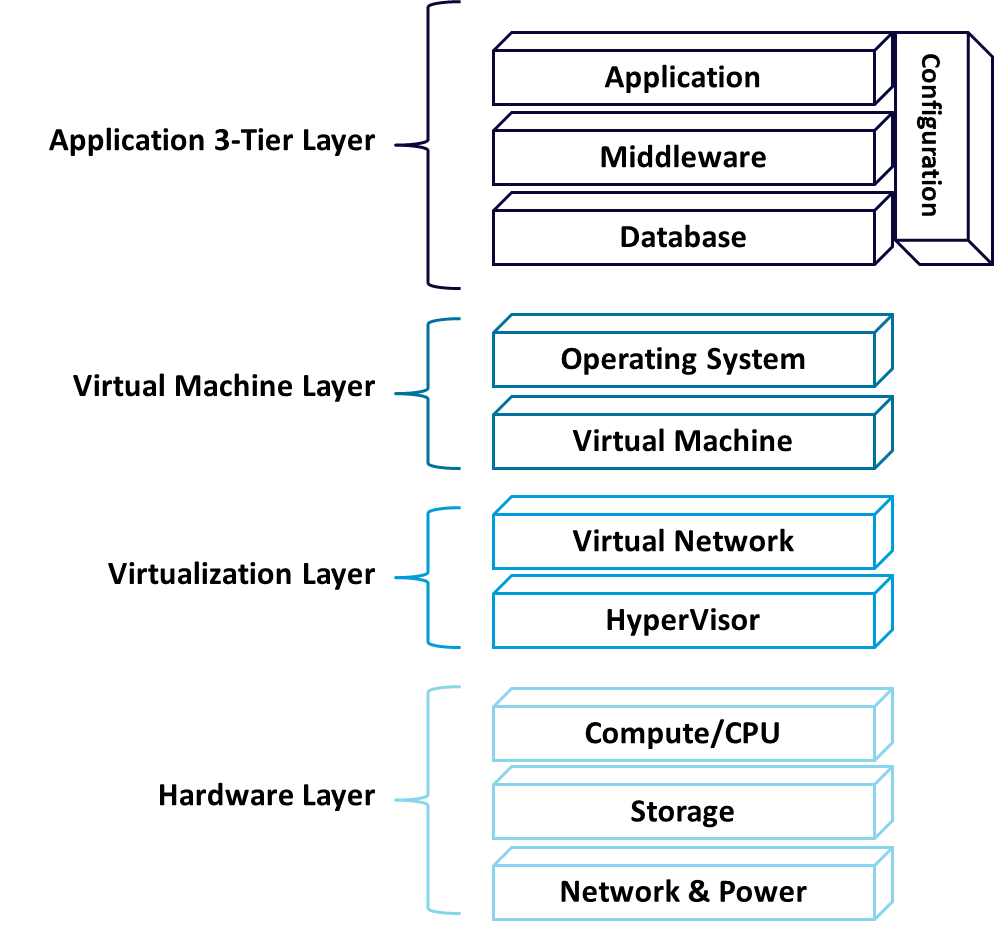
\includegraphics[width=0.6\linewidth]{osi-cloud-stack}
    \caption{OSI-Cloud Stack}
    \label{fig:osi-cloud-stack}
\end{figure}